%% This is an example first chapter.  You should put chapter/appendix that you
%% write into a separate file, and add a line \include{yourfilename} to
%% main.tex, where `yourfilename.tex' is the name of the chapter/appendix file.
%% You can process specific files by typing their names in at the 
%% \files=
%% prompt when you run the file main.tex through LaTeX.
\chapter{Results}



\section{Implementation for daWUAPhydroengine}

The \textbf{daWUAPhydroengine} hydrologic model is designed to be implemented in any geographic location. For this study it was utilized to model streamflows throughout the state of Montana. \textbf{daWUAPhydroengine} takes precipitation, minimum temperatures, and maximum temperatures as inputs and outputs streamflow data along with some additional states such as snow water equivalent. Since Montana is such a large geographical area sections of the landscape differ in various ways (soil composition, forestation, etc.) To account for this, a series of geospatially distributed raster parameters are calibrated by the filter. Since each parameter is corrected by model state predictions and observations raster images were separated into distinct theissen raster regions, each with an observation point at its center.

\begin{figure}[h]
    \centering
    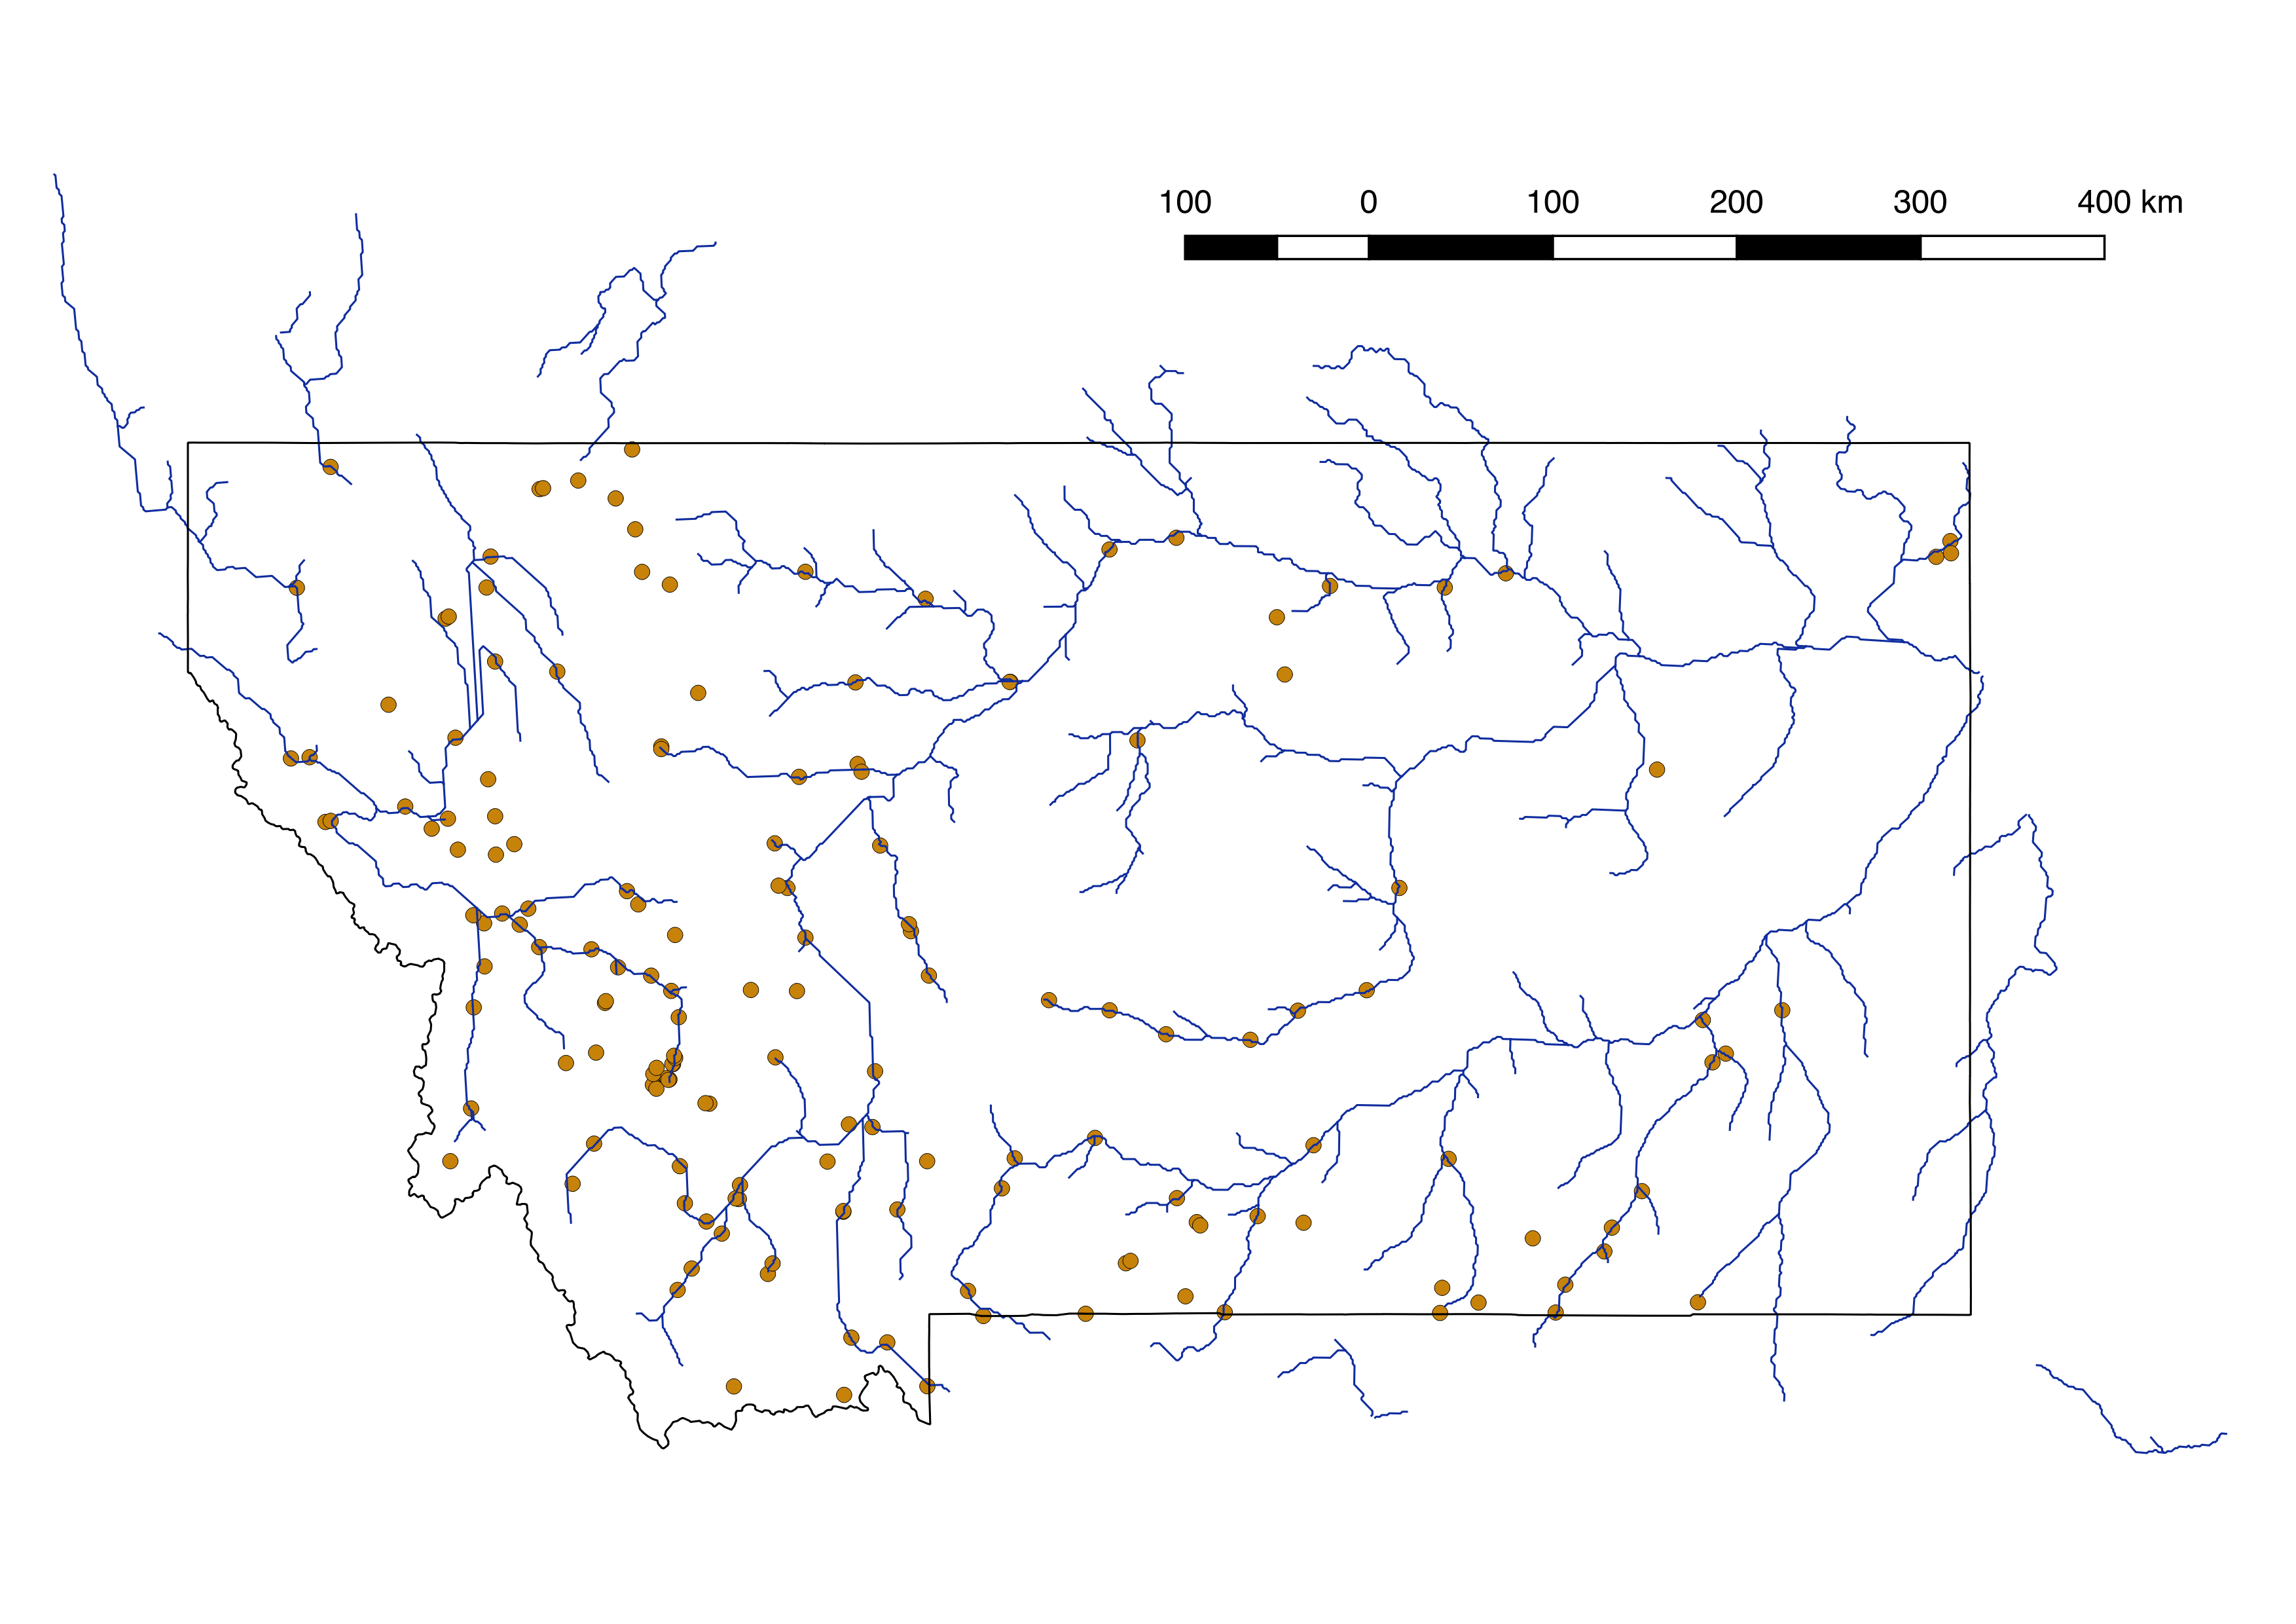
\includegraphics[width=0.95\textwidth]{stations}
    \caption{all SWE stations plotted against modeled streamflows}
    \label{fig:stations}
\end{figure}

\begin{table}[]
\caption{Calibrated Parameters} 
\begin{tabular}{lll}
Parameter ($\theta$) & Purpose                                                    & Dimensions  \\ \hline
ddf                  & Controls Rate of Snowfall                                        & 45012 \\
aet\_lp              & Controls AET                                                      & 45012 \\
soil\_beta           & Controls portion of ponded water that goes into soil storage & 45012 \\
soil\_max\_wat       & Controls soil maximum water capacity & 45012
\end{tabular}
\label{tab:t_params}
\end{table}

To apply the filter to \textbf{daWUAPhydroengine} minimum temperature, maximum temperature, and precipitation were treated as forcing data. 


\begin{table}[]
\caption{Forcing Data} 
\begin{tabular}{lll}
Forcing Data ($u$) & Purpose                          & Dimensions \\ \hline
tempmin          & Lowest temperature for timestep  & 45012 \\
tempmax          & Highest temperature for timestep & 45012 \\
precipitation      & Amount of rainfall for timestep & 45012 
\end{tabular}
\label{tab:u_params}
\end{table}


To implement the Dual Ensemble Kalman Filter with these parameters and forcing data it was necessary to set a minimum and maximum cutoff point for random perturbation (temperatures under 0 Kelvin, for example, break the filter.) Although this method worked well  for the forcing data the maximum and minimum cutoffs broke the calibrated parameters. This is because the filter would sometimes correct above or below the parameter values, which resulted in a collapse of the ensemble variance. Since ensemble variance is used to determine the variance of the next timestep's random perturbations the filter could not recover. Two solutions were implemented to keep this from happening: 1) A 'minimum variance' was specified and 2) When one or more values would be corrected past a minimum or maximum cutoff the whole ensemble would simply not correct for that iteration.

\begin{table}[]
\caption{States} 
\begin{tabular}{lll}
State ($x$) & Purpose                              & Dimensions  \\ \hline
streamflow  & Streamflow (in cumecs)               & 330   \\
swe         & Snow Water Equivalent  (in $mm^{3}$) & 45012
\end{tabular}
\label{tab:states}
\end{table}

Each run involved 100-200 ensembles and took anywhere from 20 hours to 2 days to run. The filter initially did not converge correctly when the kernel smoothing $a$ and $h$ values suggested by Moradkhani et al. were used. When the stronger set of values suggested by Chen et al. \cite{Chen2008} were used the parameters converged nicely. Although it was initially worried that stronger kernel smoothing would not allow the ensembles to converge to the correct value values seem constant and consistent with other examples of the literature.


\begin{figure}[h]
    \centering
    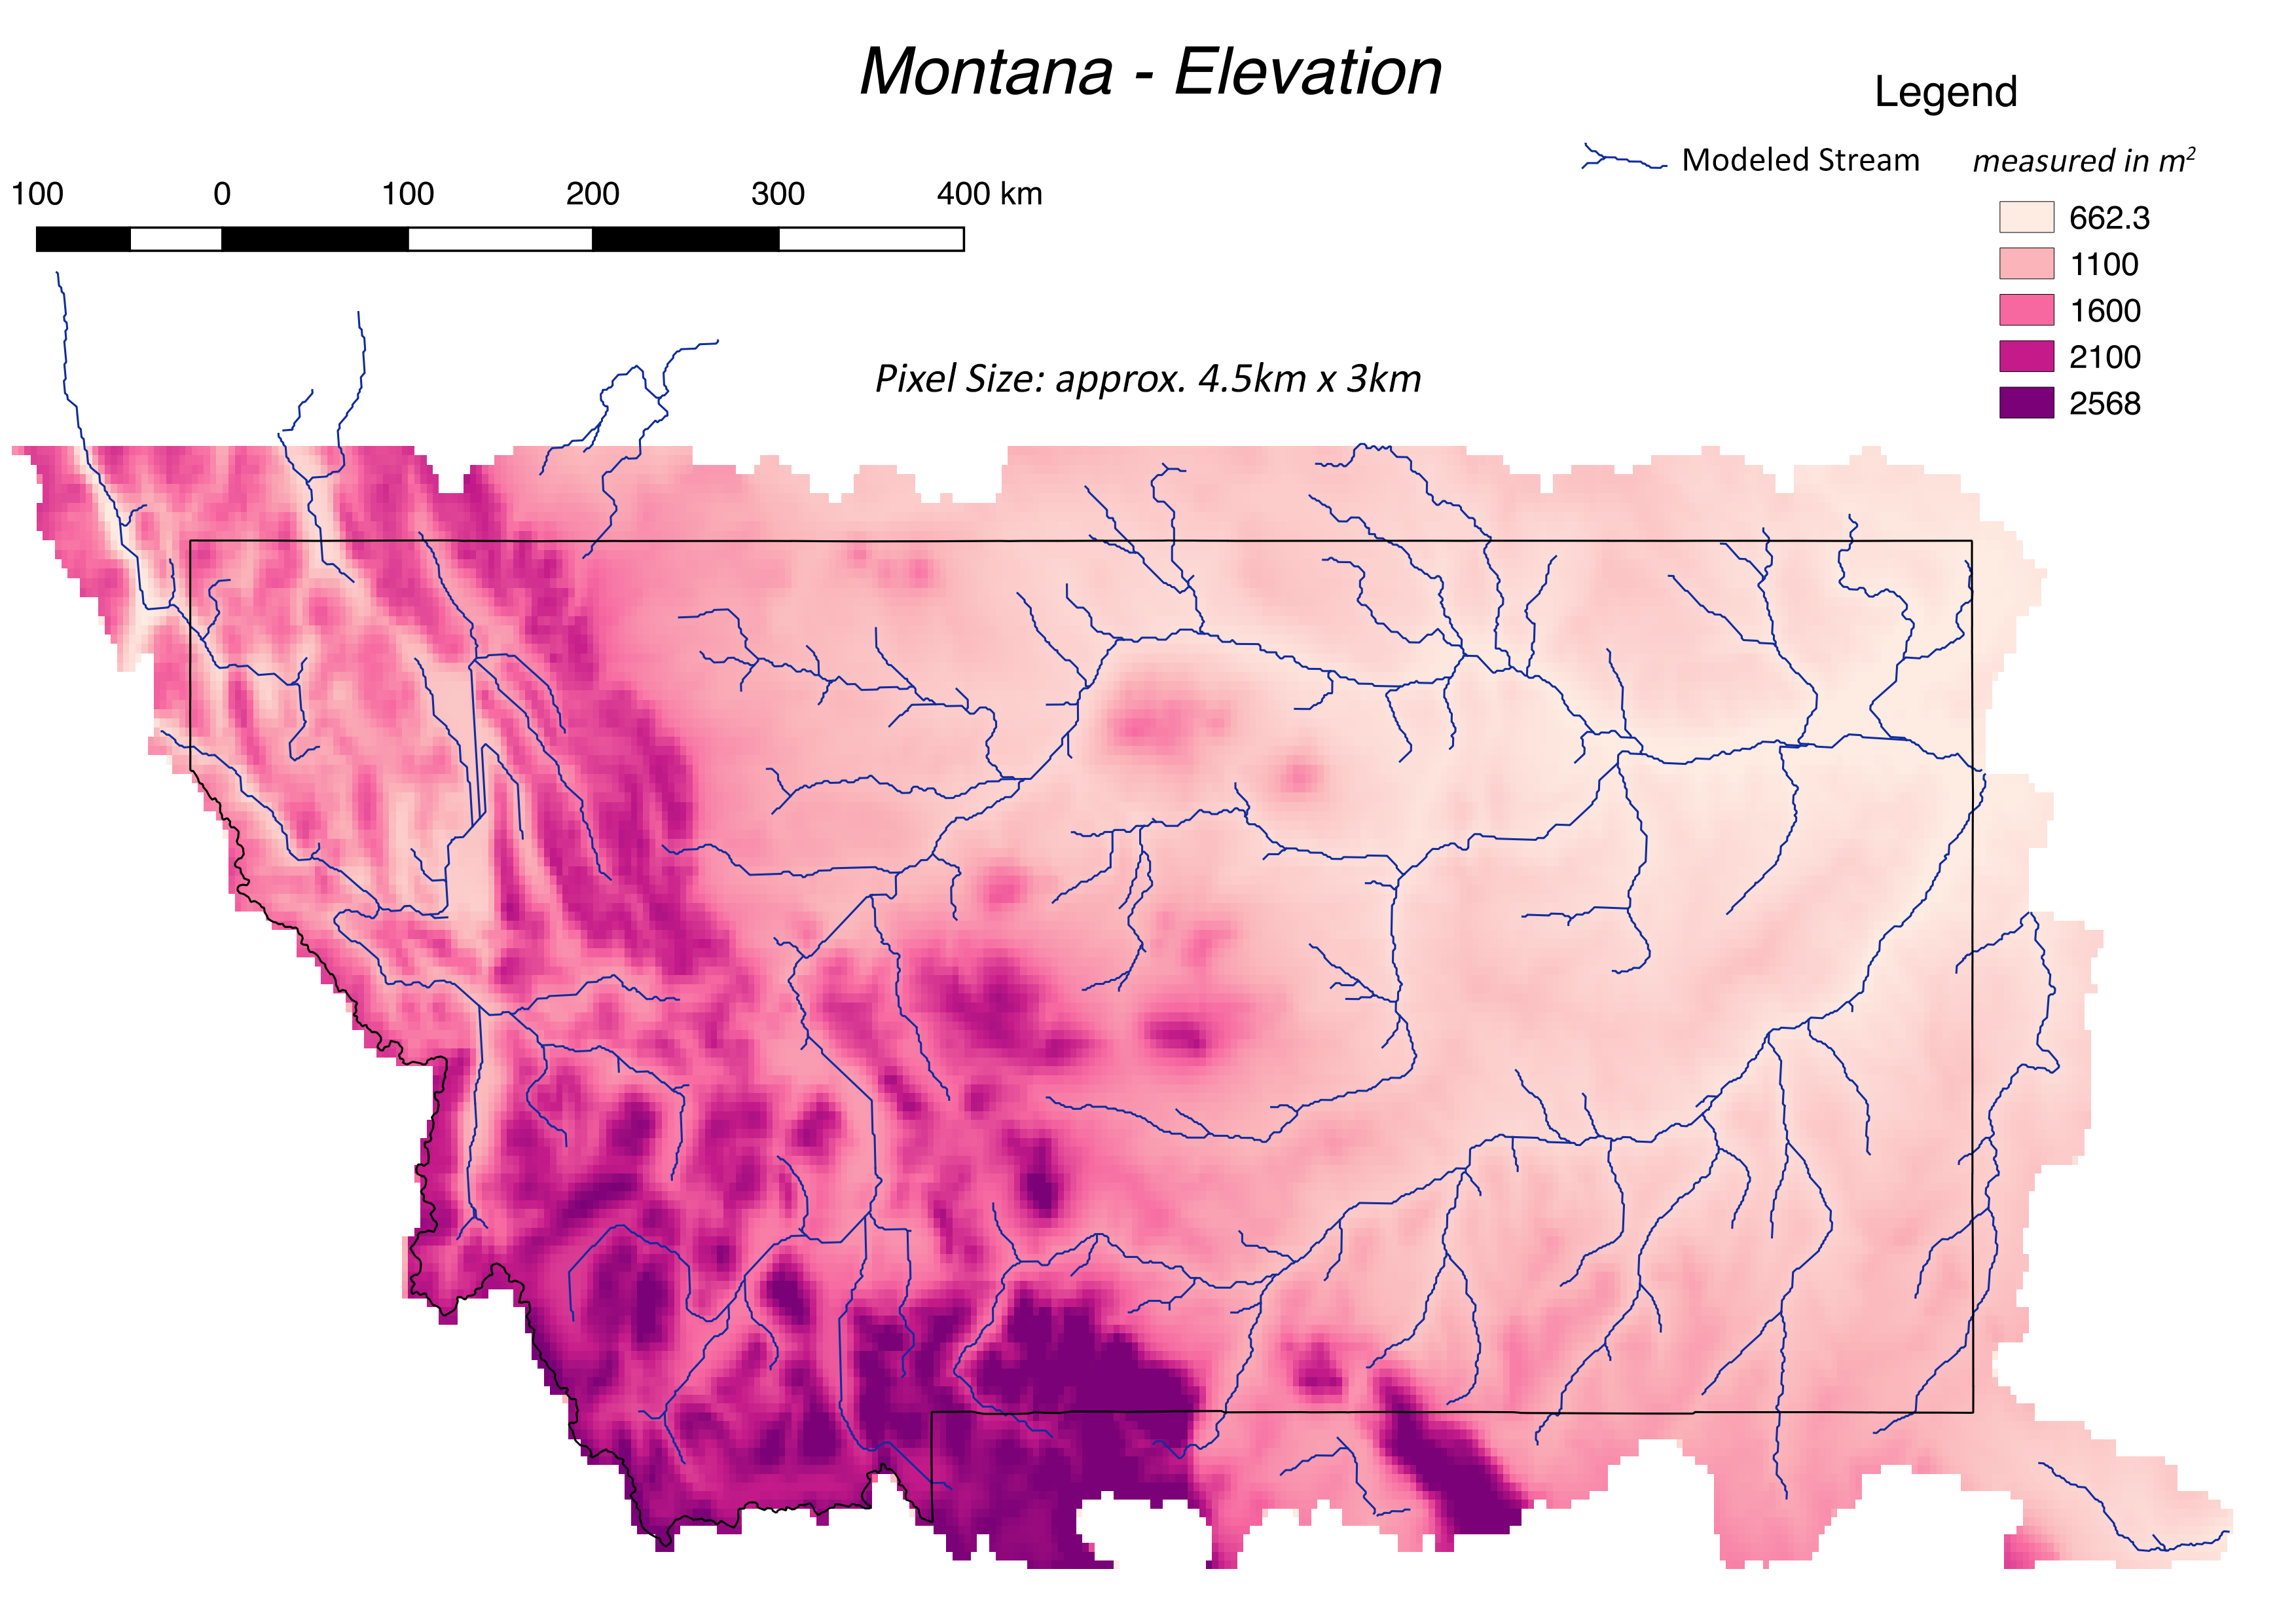
\includegraphics[width=0.95\textwidth]{elevation}
    \caption{Elevation throughout Montana}
    \label{fig:elevation}
\end{figure}

\begin{figure}[h]
    \centering
    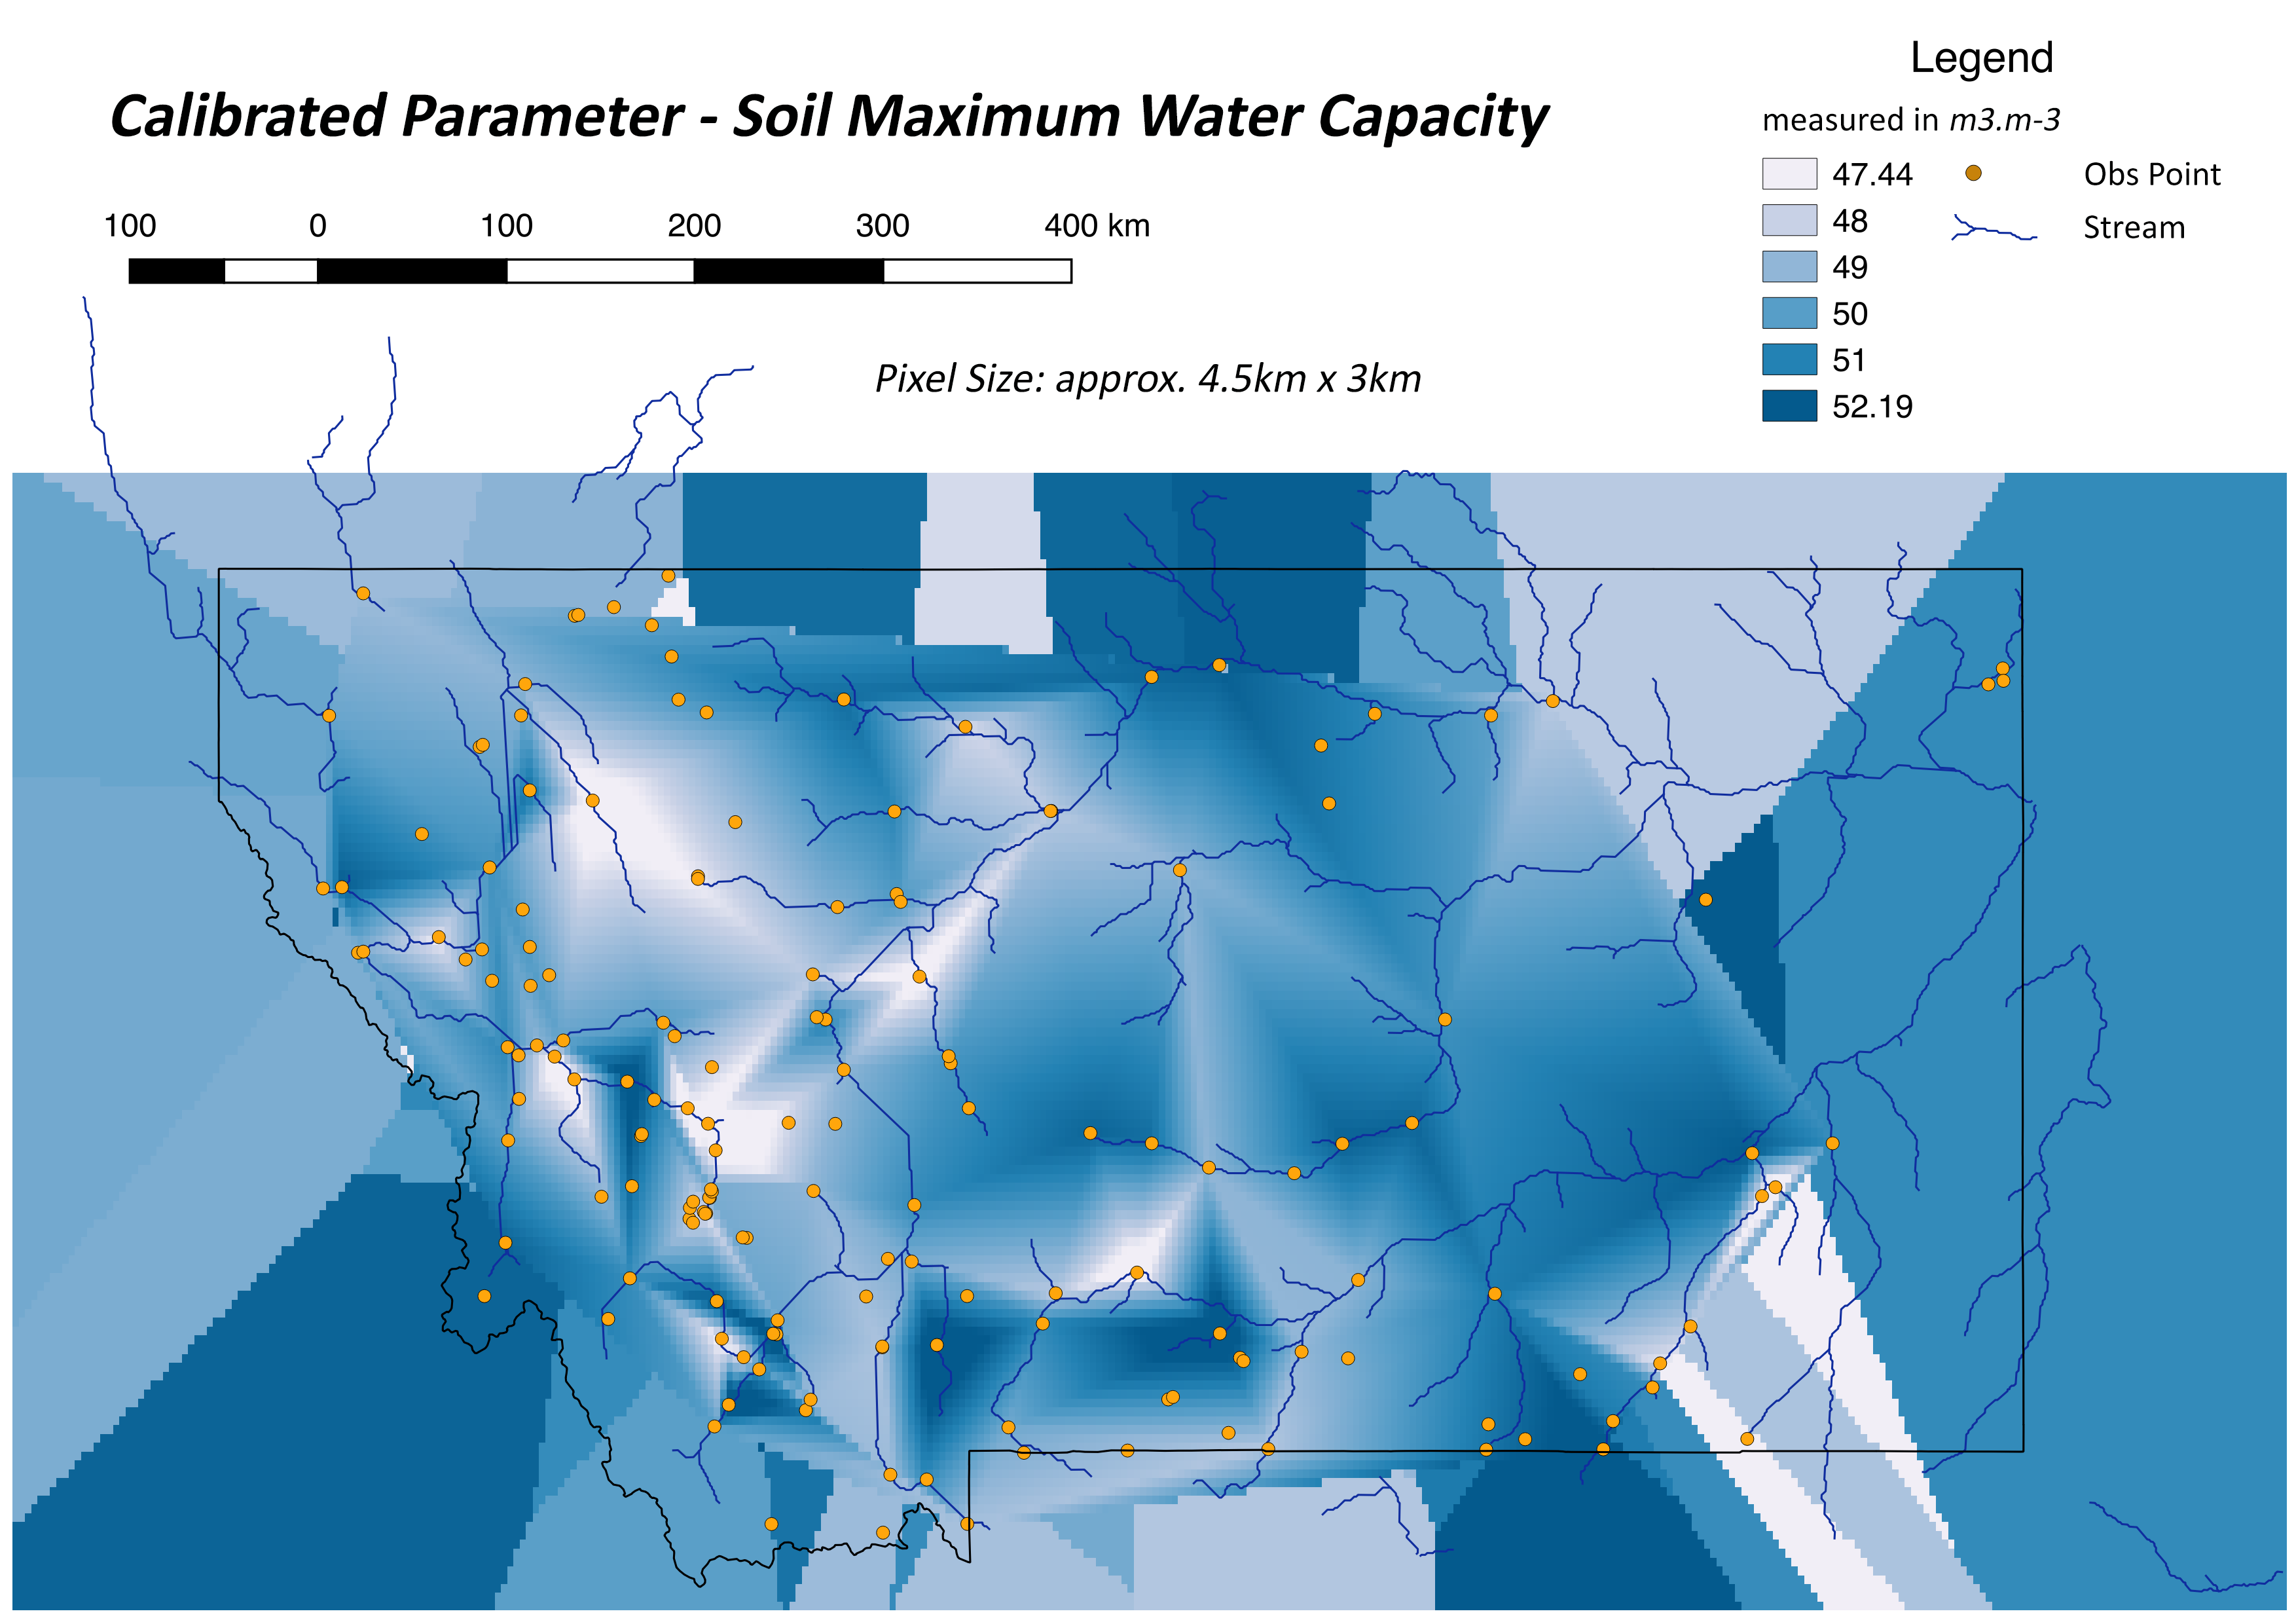
\includegraphics[width=0.95\textwidth]{max_wat}
    \caption{A calibrated raster - maximum water capacity}
    \label{fig:max_wat}
\end{figure} 

\begin{figure}[h]
    \centering
    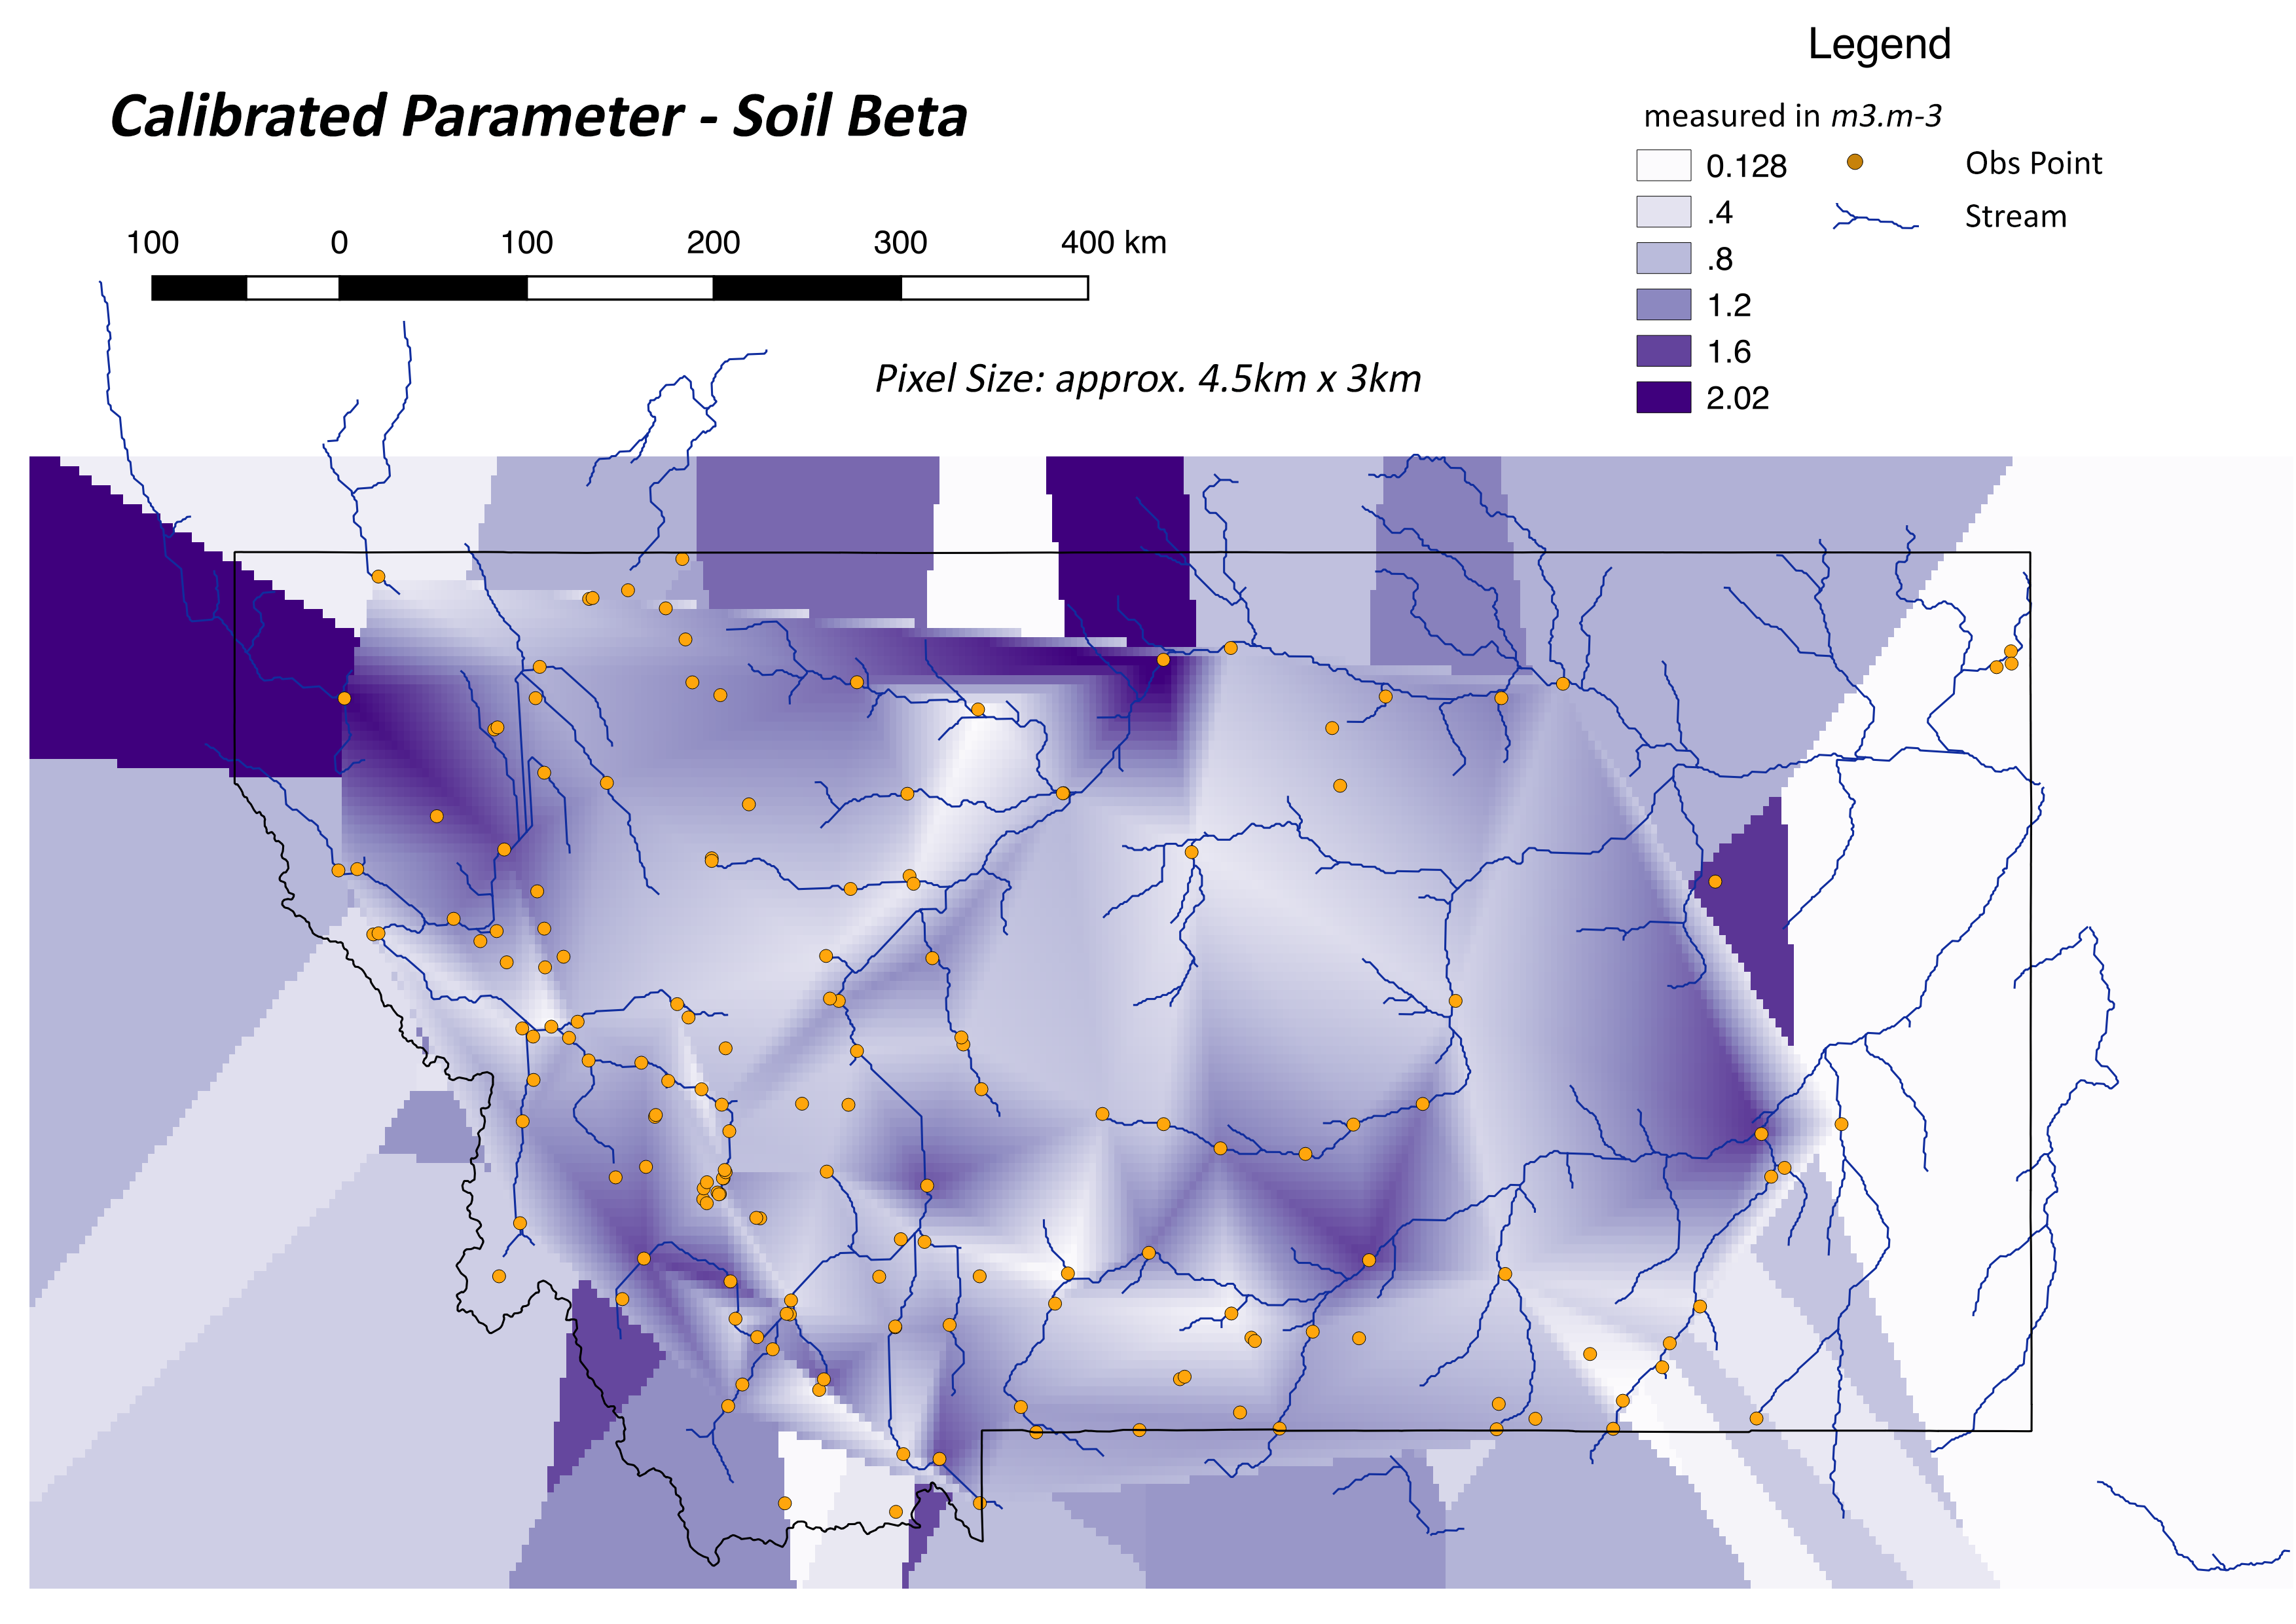
\includegraphics[width=0.95\textwidth]{soil_beta}
    \caption{A calibrated raster - maximum water capacity}
    \label{fig:soil_beta}
\end{figure} 

\ref{fig:max_wat} is a visualization of the resulting raster of the calibrated soil max water content parameter. \ref{fig:soil_beta} is a visualization of the resulting raster raster of the soil beta parameter. When contrasting these with \ref{fig:elevation} it becomes clear that these parameters are not correlated with elevation. If this was the case, it would point to a flaw in \textbf{daWUAPhydroengine}'s algorithms. Instead, parameter values are spaced evenly and do not form a trival pattern. This is optimal, as these parameters make up for real world factors that \textbf{daWUAPhydroengine}'s methods do not take into account.

\begin{figure}[h]
    \centering
    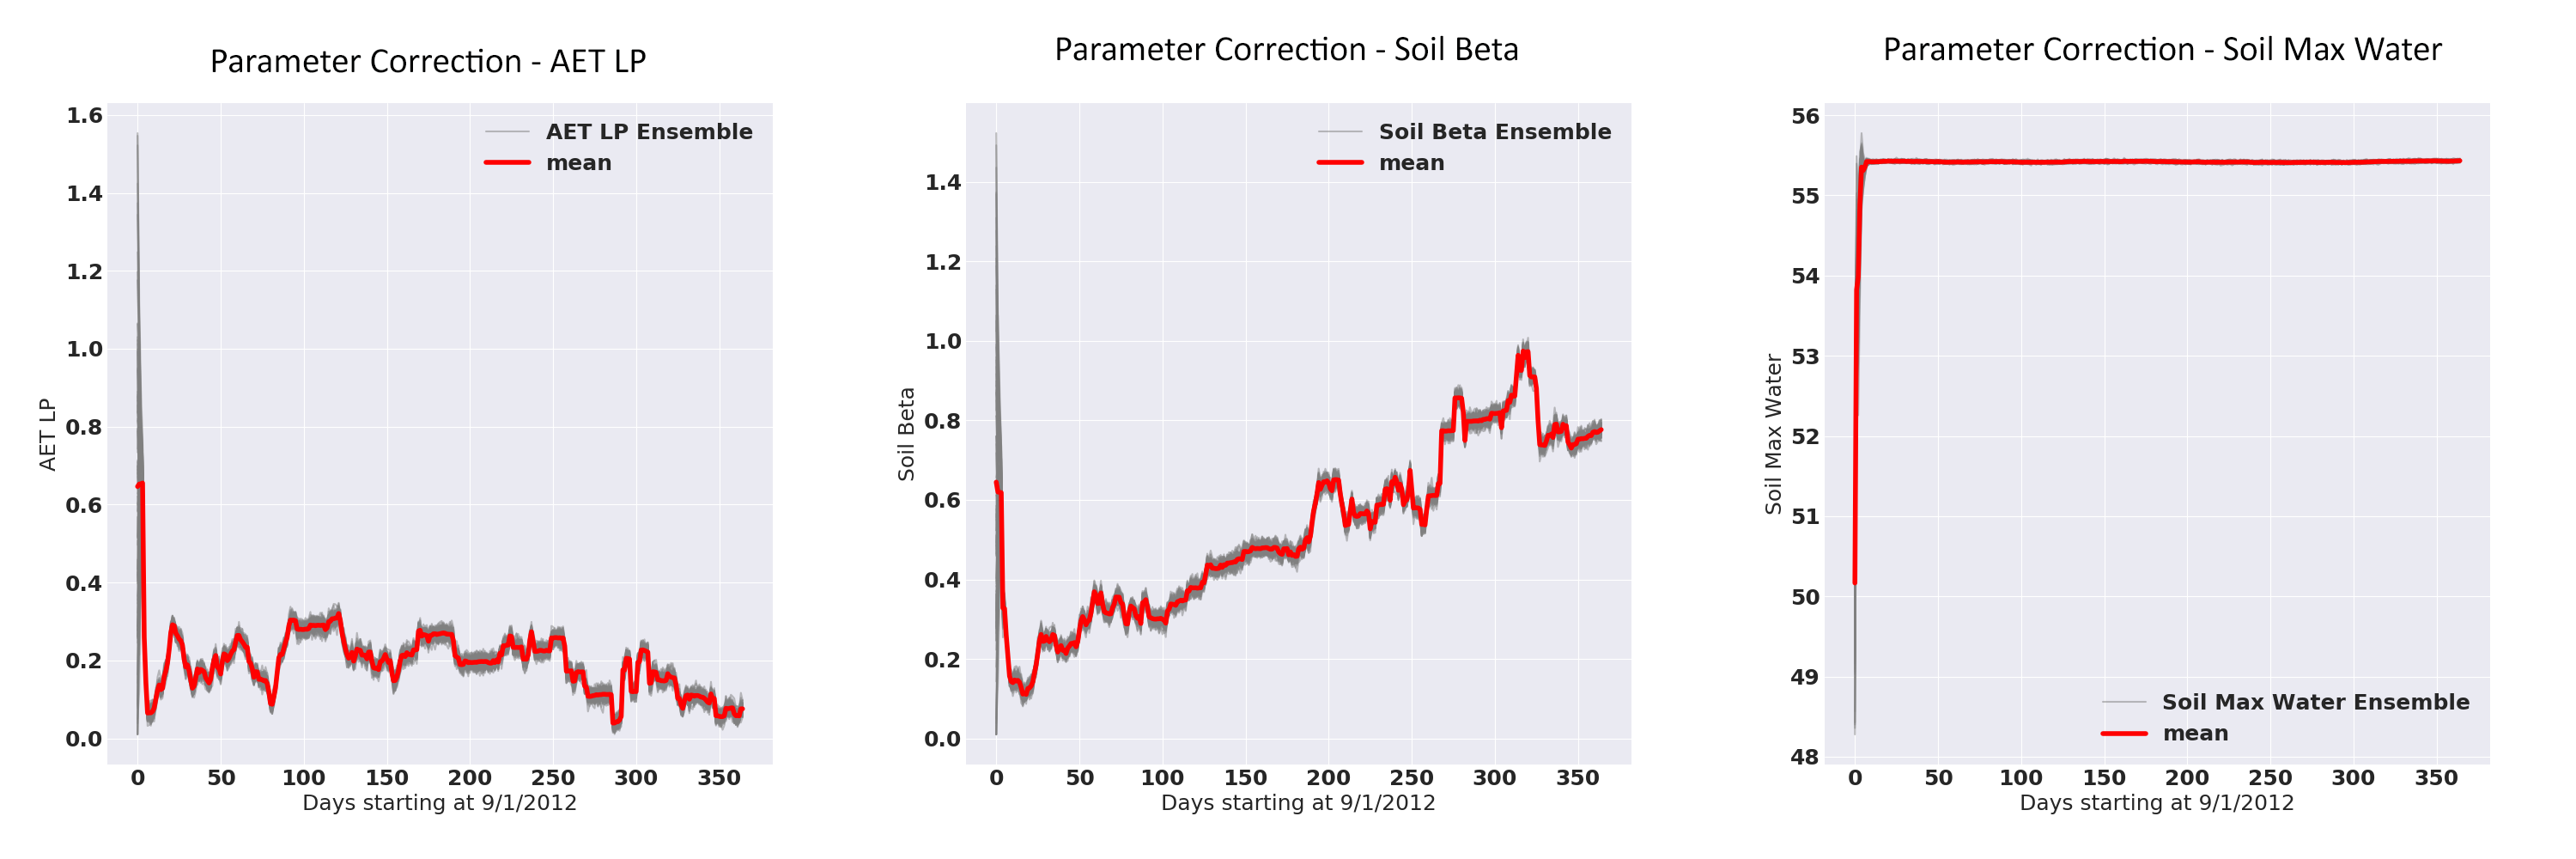
\includegraphics[width=0.95\textwidth]{param}
    \caption{Parameter convergences over time}
    \label{fig:param}
\end{figure} 

\ref{fig:param} shows the convergence process of three streamflow parameters: AET LP, Soil Beta, and Soil Max Water. The confidence interval is substituted for the ensemble cloud since the amount of perturbation per time step is derived from the variance over all ensembles. Each ensemble converges very nicely.

\begin{figure}[h]
    \centering
    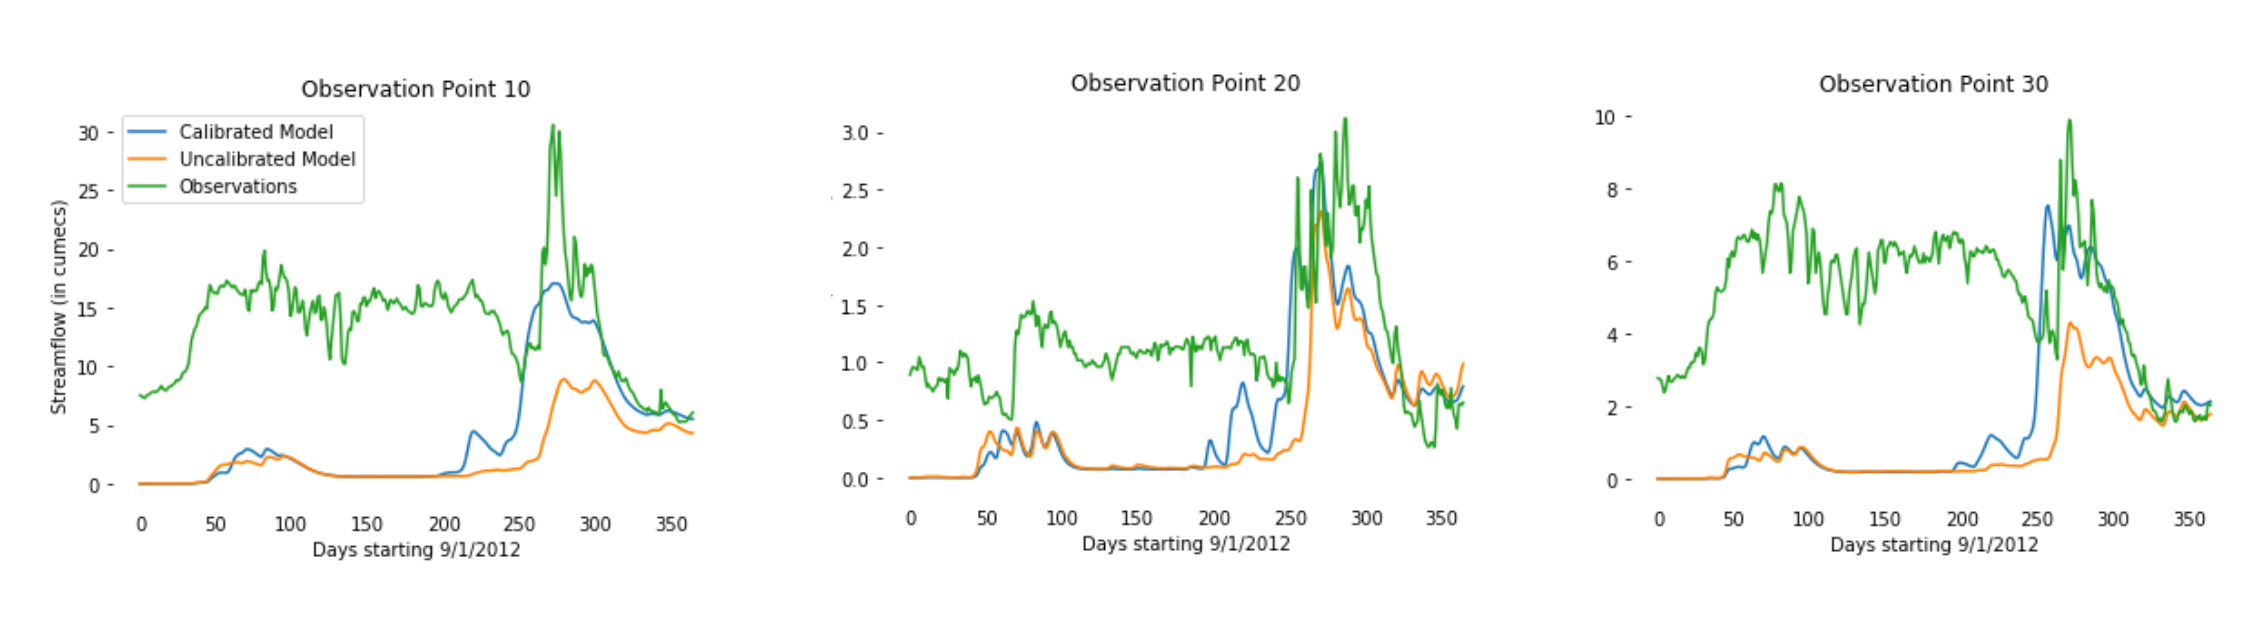
\includegraphics[width=0.95\textwidth]{cali}
    \caption{A calibrated raster - maximum water capacity}
    \label{fig:cali}
\end{figure} 

\ref{fig:cali} display stream observations compared to two instances of \textbf{daWUAPhydroengine}, one using the calibrated parameters and one using the default parameters. Both models were started without spun up parameters (e.g both models started with 0 for each streamflow and have to converge with the real world.) Note how much more successful the calibrated model behaves.

